%!TEX root = ../Thesis.tex
%\chapter{Long chapter title with $\pi$ $π$ or π}
%\chapter{Long chapter title with \texorpdfstring{$\pi$ $π$ or π}{π π or π}}
\section[Complex-valued neural networks for machine learning on non-stationary physical data]{Complex-valued\\neural networks\\for machine learning on\\\hspace*{-2cm}non-stationary physical data}

\todo{Include Abstract}
\paragraph{Abstract:} Deep learning has become an area of interest in most scientific areas, including physical sciences. Modern networks apply real-valued transformations on the data. Particularly, convolutions in convolutional neural networks discard phase information entirely. Many deterministic signals, such as seismic data or electrical signals, contain significant information in the phase of the signal. We explore complex-valued deep convolutional networks to leverage non-linear feature maps. Seismic data commonly has a lowcut filter applied, to attenuate noise from ocean waves and similar long wavelength contributions. Discarding the phase information leads to low-frequency aliasing analogous to the Nyquist-Shannon theorem for high frequencies. In non-stationary data, the phase content can stabilize training and improve the generalizability of neural networks. While it has been shown that phase content can be restored in deep neural networks, we show how including phase information in feature maps improves both training and inference from deterministic physical data. Furthermore, we show that the reduction of parameters in a complex network results in training on a smaller dataset without overfitting, in comparison to a real-valued network with the same performance.


{\vfill\hfill\newline\fbox{\parbox{.97\textwidth}{\fullcite{dramsch2019complex}}}}
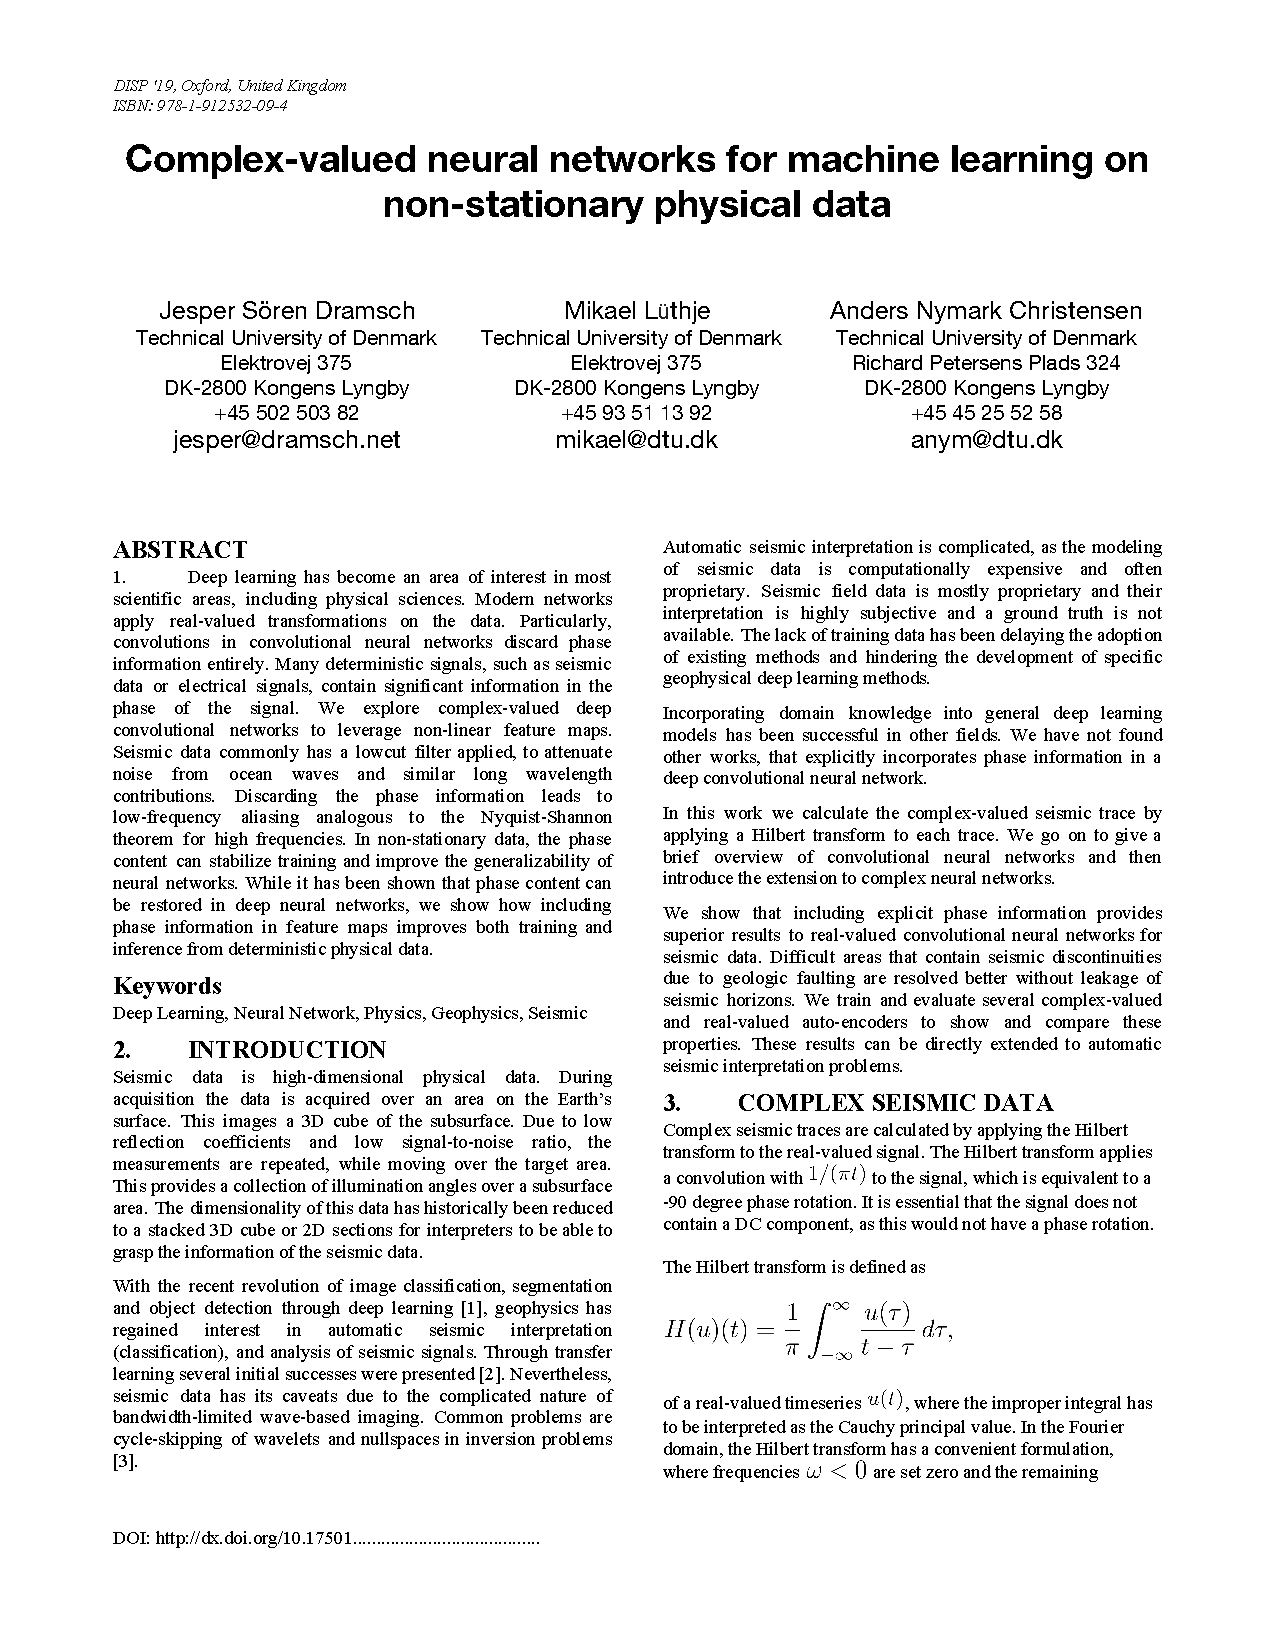
\includepdf[pages=1-6,pagecommand={},width=1.2\textwidth,offset=0.7cm 0.1cm]{papers/2019.1}
\todo{Replace Paper}
\todo{Check Page Numbers}
\todo{Fix Alignment}